% Generated by 07_plot_figure2.R -- do not edit by hand
\documentclass[12pt, border=1pt]{standalone}
\usepackage[T1]{fontenc}
\usepackage{lmodern}
\usepackage{pgfplots}
\pgfplotsset{compat=1.18}
\definecolor{c1}{HTML}{0072B2}
\definecolor{c2}{HTML}{D55E00}
\definecolor{c3}{HTML}{009E73}
\definecolor{o1}{HTML}{A9CCEB}
\definecolor{o2}{HTML}{4A90C8}
\definecolor{o3}{HTML}{0B4A7E}
\pgfplotsset{panel/.style={
  width=9.2cm, scale only axis, font=\footnotesize, set layers,
  axis line style={black!55, line width=0.4pt}, axis x line*=bottom, axis y line*=left,
  tick style={black!55, line width=0.4pt}, major tick length=2.5pt,
  y tick style={draw=none}, yticklabel style={font=\footnotesize, text=black!85},
  xticklabel style={font=\footnotesize, text=black!85}, xlabel style={font=\footnotesize, text=black!85},
  xmajorgrids, major grid style={black!12, line width=0.4pt},
  clip=false, axis on top=false, enlargelimits=false,
}}
\tikzset{title/.style={font=\small\bfseries, inner sep=0pt},
  period/.style={font=\scriptsize\itshape, text=black!60, anchor=west, xshift=4pt}}
\begin{document}
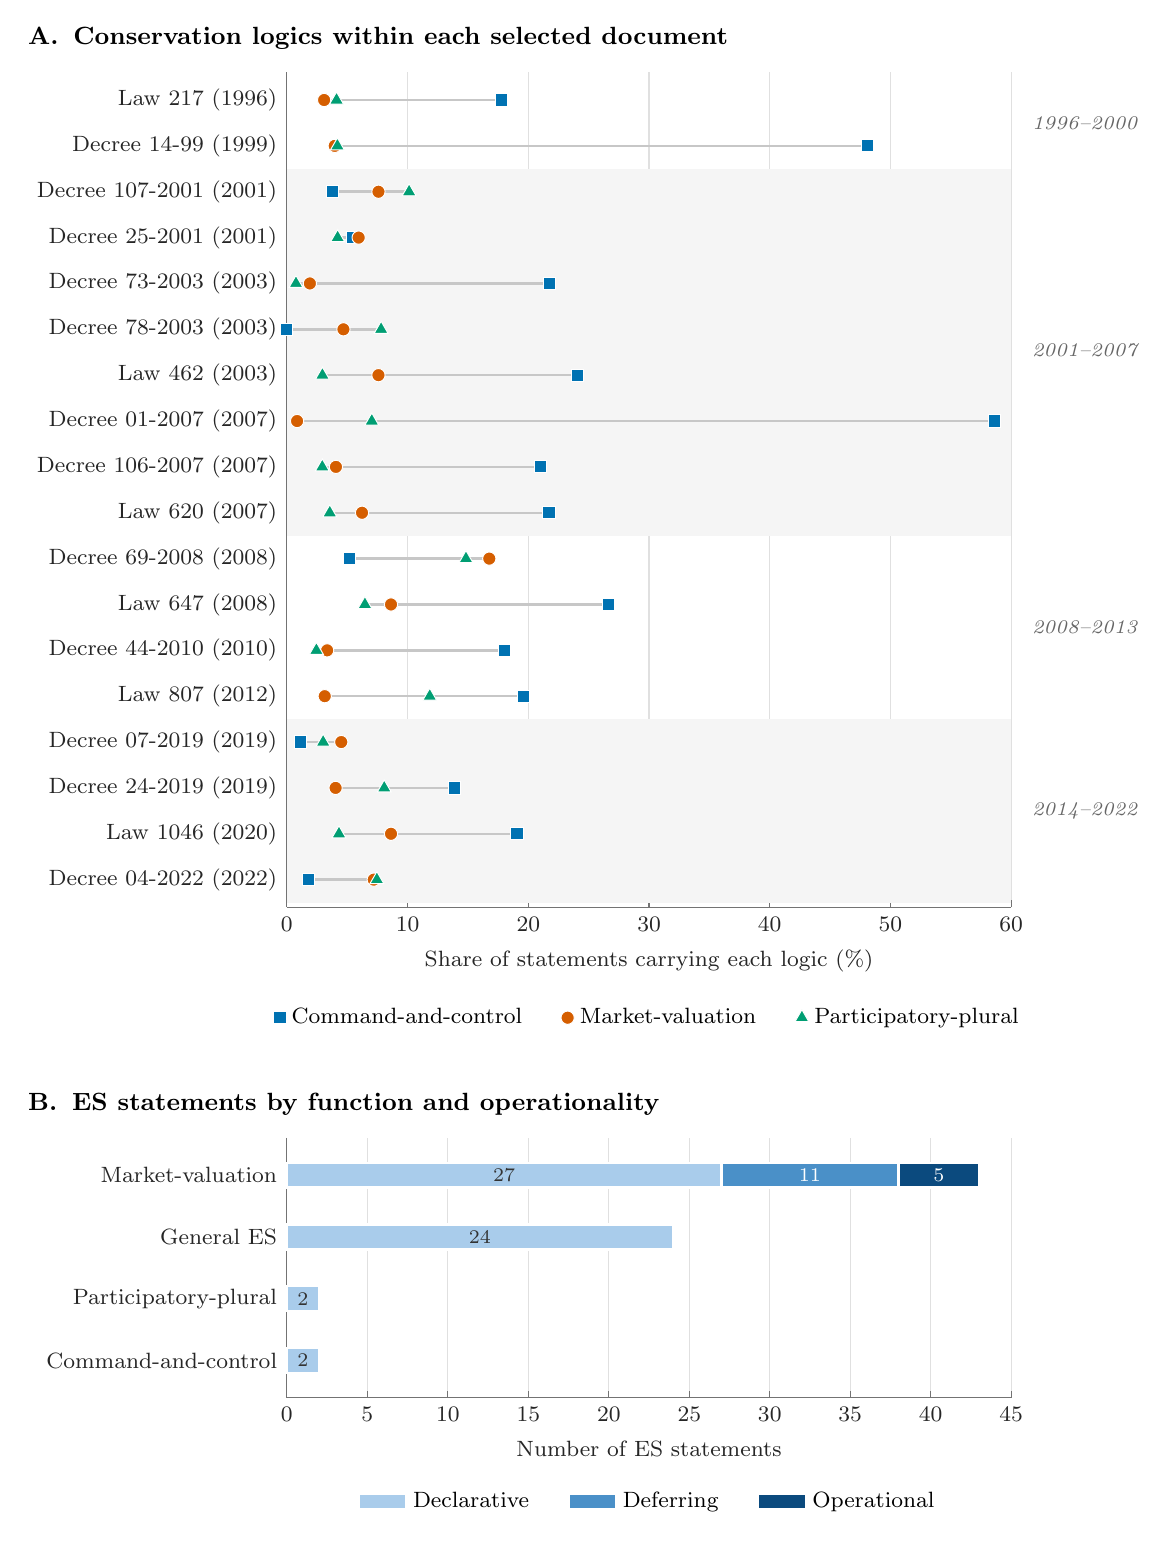
\begin{tikzpicture}
\begin{axis}[name=a, panel, height=10.6cm,
  xmin=0, xmax=60, ymin=0.4, ymax=18.6, y dir=reverse,
  ytick={1,...,18}, yticklabels={{Law 217 (1996)},{Decree 14-99 (1999)},{Decree 107-2001 (2001)},{Decree 25-2001 (2001)},{Decree 73-2003 (2003)},{Decree 78-2003 (2003)},{Law 462 (2003)},{Decree 01-2007 (2007)},{Decree 106-2007 (2007)},{Law 620 (2007)},{Decree 69-2008 (2008)},{Law 647 (2008)},{Decree 44-2010 (2010)},{Law 807 (2012)},{Decree 07-2019 (2019)},{Decree 24-2019 (2019)},{Law 1046 (2020)},{Decree 04-2022 (2022)}},
  xlabel={Share of statements carrying each logic (\%)},
  legend to name=legendA, legend columns=3,
  legend style={draw=none, font=\footnotesize, /tikz/every even column/.append style={column sep=1.2em}},
]
\node[period] at (axis cs:60,1.5) {1996--2000};
\fill[black!4] (axis cs:0,2.5) rectangle (axis cs:60,10.5);
\node[period] at (axis cs:60,6.5) {2001--2007};
\node[period] at (axis cs:60,12.5) {2008--2013};
\fill[black!4] (axis cs:0,14.5) rectangle (axis cs:60,18.5);
\node[period] at (axis cs:60,16.5) {2014--2022};
\addplot[black!22, line width=0.9pt, forget plot] coordinates {(3.09,1) (17.78,1)};
\addplot[black!22, line width=0.9pt, forget plot] coordinates {(3.97,2) (48.12,2)};
\addplot[black!22, line width=0.9pt, forget plot] coordinates {(3.80,3) (10.13,3)};
\addplot[black!22, line width=0.9pt, forget plot] coordinates {(4.21,4) (5.95,4)};
\addplot[black!22, line width=0.9pt, forget plot] coordinates {(0.76,5) (21.76,5)};
\addplot[black!22, line width=0.9pt, forget plot] coordinates {(0.00,6) (7.81,6)};
\addplot[black!22, line width=0.9pt, forget plot] coordinates {(2.95,7) (24.05,7)};
\addplot[black!22, line width=0.9pt, forget plot] coordinates {(0.85,8) (58.64,8)};
\addplot[black!22, line width=0.9pt, forget plot] coordinates {(2.94,9) (21.04,9)};
\addplot[black!22, line width=0.9pt, forget plot] coordinates {(3.56,10) (21.71,10)};
\addplot[black!22, line width=0.9pt, forget plot] coordinates {(5.16,11) (16.77,11)};
\addplot[black!22, line width=0.9pt, forget plot] coordinates {(6.47,12) (26.62,12)};
\addplot[black!22, line width=0.9pt, forget plot] coordinates {(2.45,13) (18.04,13)};
\addplot[black!22, line width=0.9pt, forget plot] coordinates {(3.14,14) (19.57,14)};
\addplot[black!22, line width=0.9pt, forget plot] coordinates {(1.13,15) (4.51,15)};
\addplot[black!22, line width=0.9pt, forget plot] coordinates {(4.04,16) (13.90,16)};
\addplot[black!22, line width=0.9pt, forget plot] coordinates {(4.32,17) (19.06,17)};
\addplot[black!22, line width=0.9pt, forget plot] coordinates {(1.80,18) (7.46,18)};
\addplot[only marks, mark=square*, mark size=2.2pt, color=c1, mark options={draw=white, line width=0.35pt}] coordinates {(17.78,1) (48.12,2) (3.80,3) (5.45,4) (21.76,5) (0.00,6) (24.05,7) (58.64,8) (21.04,9) (21.71,10) (5.16,11) (26.62,12) (18.04,13) (19.57,14) (1.13,15) (13.90,16) (19.06,17) (1.80,18)};
\addlegendentry{Command-and-control}
\addplot[only marks, mark=*, mark size=2.4pt, color=c2, mark options={draw=white, line width=0.35pt}] coordinates {(3.09,1) (3.97,2) (7.59,3) (5.95,4) (1.91,5) (4.69,6) (7.59,7) (0.85,8) (4.07,9) (6.23,10) (16.77,11) (8.63,12) (3.34,13) (3.14,14) (4.51,15) (4.04,16) (8.63,17) (7.20,18)};
\addlegendentry{Market-valuation}
\addplot[only marks, mark=triangle*, mark size=2.9pt, color=c3, mark options={draw=white, line width=0.35pt}] coordinates {(4.12,1) (4.19,2) (10.13,3) (4.21,4) (0.76,5) (7.81,6) (2.95,7) (7.04,8) (2.94,9) (3.56,10) (14.84,11) (6.47,12) (2.45,13) (11.84,14) (3.01,15) (8.07,16) (4.32,17) (7.46,18)};
\addlegendentry{Participatory-plural}
\end{axis}
\node[title, anchor=south west] at ([yshift=8pt]a.north -| a.outer west) {A.\enspace Conservation logics within each selected document};
\node[anchor=north] (la) at ([yshift=-2pt]a.outer south -| a.south) {\pgfplotslegendfromname{legendA}};
\node[title, anchor=north west] (tb) at ([yshift=-16pt]la.south -| a.outer west) {B.\enspace ES statements by function and operationality};
\coordinate (bpos) at ([yshift=-8pt]tb.south -| a.south west);
\begin{axis}[name=b, panel, at={(bpos)}, anchor=north west, height=3.3cm,
  xbar stacked, bar width=9pt, xmin=0, xmax=45, ymin=0.4, ymax=4.6, y dir=reverse,
  ytick={1,...,4}, yticklabels={{Market-valuation},{General ES},{Participatory-plural},{Command-and-control}},
  xlabel={Number of ES statements},
  legend to name=legendB, legend columns=3, area legend,
  legend style={draw=none, font=\footnotesize, /tikz/every even column/.append style={column sep=1.2em}},
  after end axis/.code={
    \node[font=\scriptsize, text=black!80] at (axis cs:13.50,1) {27};
    \node[font=\scriptsize, text=white] at (axis cs:32.50,1) {11};
    \node[font=\scriptsize, text=white] at (axis cs:40.50,1) {5};
    \node[font=\scriptsize, text=black!80] at (axis cs:12.00,2) {24};
    \node[font=\scriptsize, text=black!80] at (axis cs:1.00,3) {2};
    \node[font=\scriptsize, text=black!80] at (axis cs:1.00,4) {2};
  },
]
\addplot[fill=o1, draw=white, line width=0.8pt] coordinates {(27,1) (24,2) (2,3) (2,4)};
\addlegendentry{Declarative}
\addplot[fill=o2, draw=white, line width=0.8pt] coordinates {(11,1) (0,2) (0,3) (0,4)};
\addlegendentry{Deferring}
\addplot[fill=o3, draw=white, line width=0.8pt] coordinates {(5,1) (0,2) (0,3) (0,4)};
\addlegendentry{Operational}
\end{axis}
\node[anchor=north] at ([yshift=-2pt]b.outer south -| b.south) {\pgfplotslegendfromname{legendB}};
\end{tikzpicture}
\end{document}
